% $Id: template.tex 11 2007-04-03 22:25:53Z jpeltier $

%\documentclass{vgtc}                          % final (conference style)
\documentclass[review]{vgtc}                 % review
%\documentclass[widereview]{vgtc}             % wide-spaced review
%\documentclass[preprint]{vgtc}               % preprint
%\documentclass[electronic]{vgtc}             % electronic version
\let\ifpdf\relax

%% Uncomment one of the lines above depending on where your paper is
%% in the conference process. ``review'' and ``widereview'' are for review
%% submission, ``preprint'' is for pre-publication, and the final version
%% doesn't use a specific qualifier. Further, ``electronic'' includes
%% hyperreferences for more convenient online viewing.

%% Please use one of the ``review'' options in combination with the
%% assigned online id (see below) ONLY if your paper uses a double blind
%% review process. Some conferences, like IEEE Vis and InfoVis, have NOT
%% in the past.

%% Figures should be in CMYK or Grey scale format, otherwise, colour 
%% shifting may occur during the printing process.

%% These three lines bring in essential packages: ``mathptmx'' for Type 1 
%% typefaces, ``graphicx'' for inclusion of EPS figures. and ``times''
%% for proper handling of the times font family.

\usepackage{mathptmx}
\usepackage{graphicx}
\usepackage{times}

%% Packages used by us
\usepackage{color}
\usepackage{caption}
\usepackage{subcaption}
\usepackage{tabularx}

%% Useful definitions
\def\tweakedsim{\raise.17ex\hbox{$\scriptstyle\sim$}}

%% We encourage the use of mathptmx for consistent usage of times font
%% throughout the proceedings. However, if you encounter conflicts
%% with other math-related packages, you may want to disable it.

%% If you are submitting a paper to a conference for review with a double
%% blind reviewing process, please replace the value ``0'' below with your
%% OnlineID. Otherwise, you may safely leave it at ``0''.
\onlineid{1519}

%% declare the category of your paper, only shown in review mode
\vgtccategory{Research}

%% allow for this line if you want the electronic option to work properly
\vgtcinsertpkg

%% In preprint mode you may define your own headline.
%\preprinttext{To appear in an IEEE VGTC sponsored conference.}

%% Paper title.

\title{Real-time Visualization of Protein Surface Features\\in Molecular Dynamics}

%% This is how authors are specified in the conference style

%% Author and Affiliation (single author).
%%\author{Roy G. Biv\thanks{e-mail: roy.g.biv@aol.com}}
%%\affiliation{\scriptsize Allied Widgets Research}

%% Author and Affiliation (multiple authors with single affiliations).
%%\author{Roy G. Biv\thanks{e-mail: roy.g.biv@aol.com} %
%%\and Ed Grimley\thanks{e-mail:ed.grimley@aol.com} %
%%\and Martha Stewart\thanks{e-mail:martha.stewart@marthastewart.com}}
%%\affiliation{\scriptsize Martha Stewart Enterprises \\ Microsoft Research}

%% Author and Affiliation (multiple authors with multiple affiliations)
\author{Roy G. Biv\thanks{e-mail: roy.g.biv@aol.com}\\ %
        \scriptsize Starbucks Research %
\and Ed Grimley\thanks{e-mail:ed.grimley@aol.com}\\ %
     \scriptsize Grimley Widgets, Inc. %
\and Martha Stewart\thanks{e-mail:martha.stewart@marthastewart.com}\\ %
     \parbox{1.4in}{\scriptsize \centering Martha Stewart Enterprises \\ Microsoft Research}}

%% A teaser figure can be included as follows, but is not recommended since
%% the space is now taken up by a full width abstract.
\teaser{
  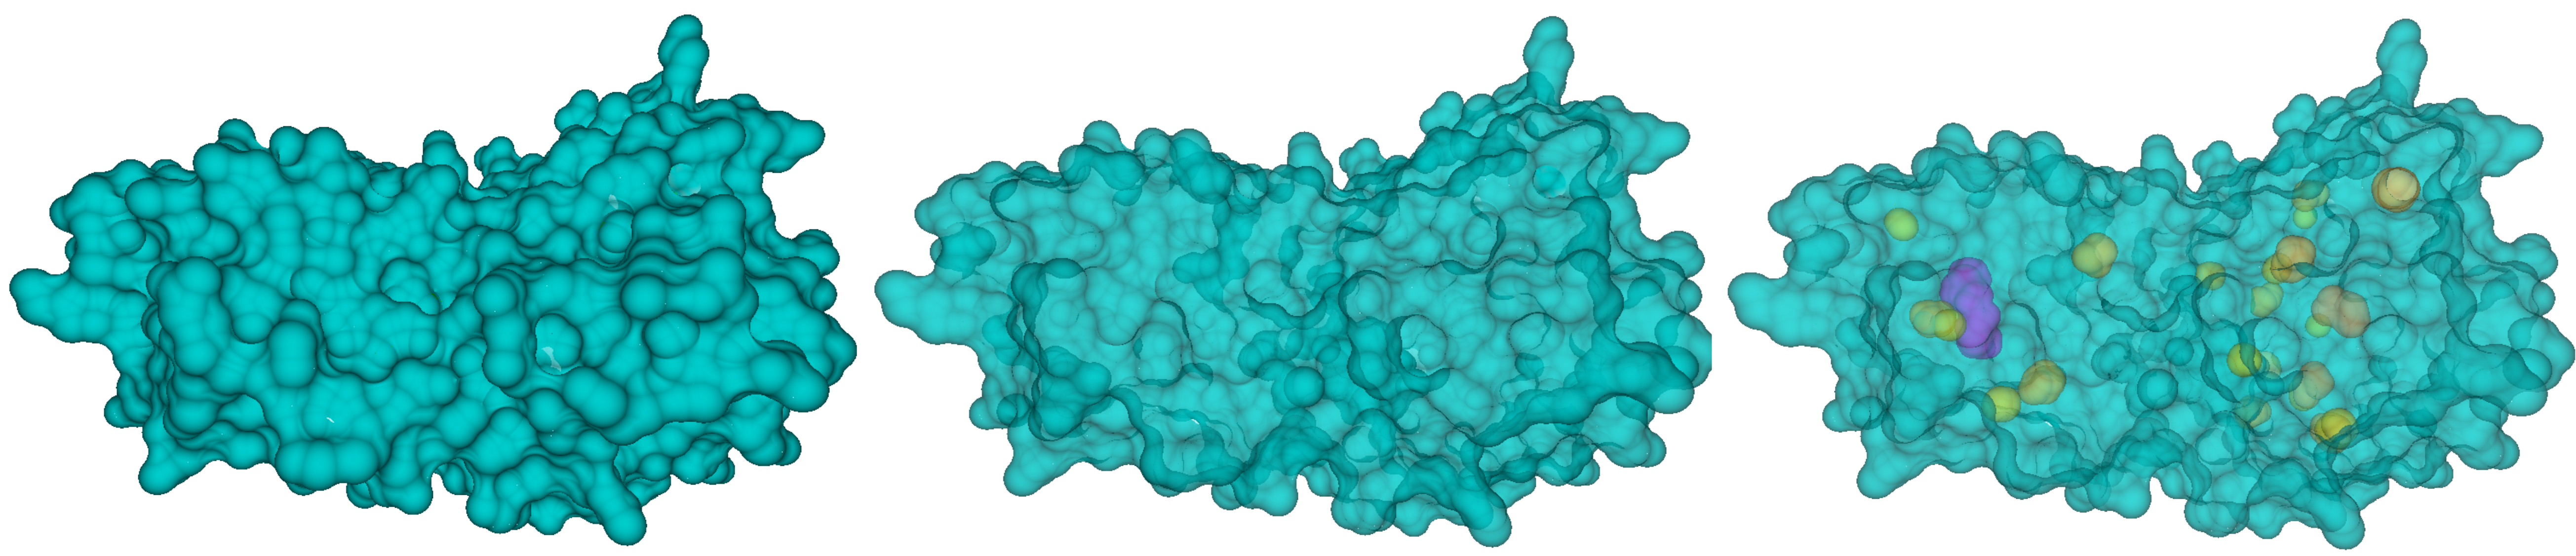
\includegraphics[width=\linewidth]{image/teaser2.png}
  \caption{An example of protein 1VIS demonstrating our visualization method. Left: The full SES model. Middle: Enabling basic transparency. c) A user defined transparent visualization that includes cavities.}
	\label{fig:teaser}
}

%% Abstract section.
\abstract{The reactivity of the biomolecular structures is highly influenced by their structural features. 
Thus, studying these features along with the exploration of their dynamic behavior helps to understand the processes ongoing in living cells.
This can be reached by the visual representation of these processes as visualization is one of the most natural ways to convey such information.
However, none of the currently available techniques provides the biochemists with an intuitive real-time representation of the dynamic movements of molecules and precise geometrical based extraction of their structural features performed instantly.
In this paper we introduce such a technique enabling the user to compute and also to visualize the molecular surface along with inner voids.
To obtain a better insight into the molecule, our technique enables to visualize the molecular surface transparently. 
The opacity can be adjusted by changing user-defined parameters in order to enhance the perception of the surfaces of inner voids.
%The whole visualization is created in a focus and context visualization manner, where the user can interactively choose the structures of interest.
All integrated algorithms run in real-time which gives the user a big variety of exploration possibilities.
The importance of our approach is even amplified with respect to the fact that currently the size of molecular dynamics simulations is increasing dramatically and offline rendering thus becomes impracticable. 
The usability of our technique is demonstrated by a case study which reflects real problems of the domain experts.
} % end of abstract

%% ACM Computing Classification System (CCS). 
%% See <http://www.acm.org/class/1998/> for details.
%% The ``\CCScat'' command takes four arguments.

\CCScatlist{
  \CCScat{I.3.5}{Computational Geometry and Object Modeling}{}Boundary representations;
  \CCScat{I.3.7}{Three-Dimensional Graphics and Realism}{}Visible line/surface algorithms
}

%% Copyright space is enabled by default as required by guidelines.
%% It is disabled by the 'review' option or via the following command:
% \nocopyrightspace

%%%%%%%%%%%%%%%%%%%%%%%%%%%%%%%%%%%%%%%%%%%%%%%%%%%%%%%%%%%%%%%%
%%%%%%%%%%%%%%%%%%%%%% START OF THE PAPER %%%%%%%%%%%%%%%%%%%%%%
%%%%%%%%%%%%%%%%%%%%%%%%%%%%%%%%%%%%%%%%%%%%%%%%%%%%%%%%%%%%%%%%%

\begin{document}

%% The ``\maketitle'' command must be the first command after the
%% ``\begin{document}'' command. It prepares and prints the title block.

%% the only exception to this rule is the \firstsection command
\firstsection{Introduction}

\maketitle

%% \section{Introduction}
Contribution
\begin{itemize}
  \item Transparent surface rendering speedup (AJ)
	\item Novel real-time cavity detection method (AJ)
	\item More precise (analytic computation + ray-casting) interactive visualization of cavities in molecular simulations (JP)
	\begin{itemize}
		\item Focus and context visualization of cavities within transparent molecular surfaces
		\item Opacity modulation by cavity features (surface area, AO, etc.)
	\end{itemize}
	\item ? Memory efficient CB (AJ)
	\item ? Vendor independent implementation (OpenGL + OpenCL) (AJ)
\end{itemize}

Problem
\begin{itemize}
  \item Artifacts \& occlusion, e.g. for secondary structures (AJ)
\end{itemize}

Nafuknut na catch up with big data analysis from MD simulation... (JP)
The exploratory process of MD simulations is often concerned with the visual identification of binding sites of ligands to a host macromolecule. These sites represent a molecular surface feature known as cavities, pockets or as tunnels. There is a legacy of tools and approaches that allow us to extract these features. Two major challenges in regards to the surface features, like cavities, are their fast extraction and their visualization in the most informative manner. This is especially crucial when analyzing MD simulations containing thousands of frames. Here, it would be ideal to have a technique that could provide us an instant computation and an interactive, and the same time clever, visualization of the cavities in the context of molecular surface. In this paper, we introduce visualization technique that enables to  ….
The contributions are as follows:
\begin{itemize}
  \item An enhanced computation of SES
  \item A novel real time algorithm for detection of cavities (check Totrov --- AJ)
  \item Focus and context visualization of cavities in the context of molecular surface
  \item Improved performance of visualization of transparent molecular surfaces
\end{itemize}

\section{Related Work}
Our approach touches several research areas, including computation and visualization of protein cavities and their surfaces. 
Further we focus on the real-time visualization of surfaces and an ambient occlusion technique enhancing the depth perception of the molecular surface. 
Thus in this section we describe the existing techniques related to these topics.

\subsection{Extraction and Visualization of Surfaces of Molecules and Their Cavities}
There are several types of molecular surface representation proposed in the literature~\cite{STAR2015}. 
However, for the cavity analysis,  the solvent-excluded surface (SES) is the most commonly used representation used by the domain experts.%~\cite{todo}. 
This representation allows us to directly asses whether a solvent, approximated by a sphere of a given radius, is able to reach a binding site of interest on the molecular surface. 

The area of geometrical analysis of molecular structures focusing on the detection and further exploration of the void space is very vast and so we do not aim to provide the users with an exhaustive list of the existing solutions. 
Rather we focus on the techniques which we consider to be the closest to our work.

The molecular surface is one of the most significant studied features thus many solutions were published.
Here we focus on the analytical approaches for the construction of the SES where Connolly~\cite{connolly1983analytical} presented the first solution to this problem.
Another approach to the detection of the analytic surface was later presented by Totrov and Abagyan~\cite{totrov1996contour}.
The algorithm is based on the sequential build up of multi-arc contours. 
One of the advantages of this contour-buildup approach is that it is localized thus applicable on the computation of partial molecular surface.

One of the significant improvements of the SES computation was published by Parulek and Viola~\cite{parulek2012implicit}.
Their approach does not require any precomputation. 
It is based on the theory of implicit surfaces where the value of the implicit function helps to determine the inner and outer points with respect to the surface.
The implicit function is composed of three types of patches from which the SES is constructed.

However, none of these solutions dealt with molecular dynamics. 
Krone et al.~\cite{krone2009interactive} presented their approach to the visualization of the SES using GPU ray casting technique which allowed to achieve interactive frame rates. \textcolor{red}{TODO: how it is in comparison with our solution?} 
Another approach by Lindow et al.~\cite{lindow2010accelerated} even accelerates the construction of the SES by scaling the parallel contour-buildup algorithm to more GPU cores and using boundary quadrangles as rasterization primitives. \textcolor{red}{TODO: how it is in comparison with our solution?}

Similarly, the analytical approaches are applicable to the protein inner voids. 
We focus only on the analytical computation and visualization of cavities which can contain a potential protein binding site.
Parulek et al.~\cite{parulek2013visual} presented their approach to the computation and visual analysis of cavities in simulations of molecular dynamics.
The computation is based on implicit function. 
The subsequent exploration is supported by graph based visualizations.
\textcolor{red}{TODO: what else?}


\subsection{Order-Independent Transparency}
\cite{carpenter1984abuffer}
\cite{everitt2001interactive}
\cite{bavoil2008order}
\cite{yang2010real}
\cite{enderton2011stochastic}
\cite{salvi2011adaptive}
\cite{maule2012memory}%star
PUXELS \cite{kauker2013rendering}


\subsection{Ambient Occlusion}
Ambient occlusion is one of the most popular techniques for enhancement of the depth perception in molecular visualization.
Tarini et al.~\cite{tarini2006ambient} as first used this technique for real-time molecular visualization.
As this technique is computationally very demanding, several solutions focusing on this limitation appeared.
Grottel et al.~\cite{grottel2012object} presented their method reaching interactive frame rates for large and dynamic data sets. 
Recently, their approach was extended by~\cite{staib2015ambient}.
This method is applicable to transparent particles as well.
Ambient occlusion technique was used also by Borland\cite{borland2011ambient} for enhancing the understanding of the interior of the molecular structure.
His technique, called ambient occlusion opacity mapping, enables to determine a variable opacity at each point on the molecular surface.
In consequence, the interior structures can be more opaque than the outer structures, i.e., molecular surface.
Because of the very convincing visual results, we employed this transparency modulation technique to our solution as well.


\begin{itemize}
  \item \textcolor{red}{Performance drop of SES rendering on newer hardware (GF 680 GTX) --- we can perform better. We contacted authors, they do not know exactly why, they think it is change in the internal architecture between Fermi and Kepler (AJ)}
  \item \textcolor{red}{Slow rendering of SAS. Too many layers in pixels --- we can do better by surface layers detection (AJ)}
\end{itemize}

\textcolor{red}{There are more solutions taken from computer graphics; e.g., OIT (JP)}

%Such binding site can be located inside a cavity or a tunnel, while the molecular surface might contain tens of cavities per single simulation time step. 




\section{Overview}
\begin{figure*}[tb]
  \centering
  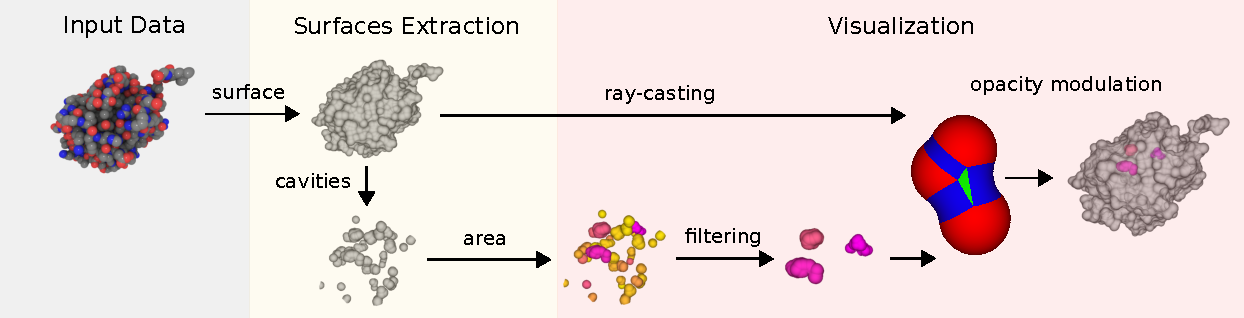
\includegraphics[width=\textwidth]{image/overview_final.pdf}
  \caption{Illustration of the visualization pipeline. The input data (Chapter~\ref{ch:overview}) contains snapshots of MD trajectories which are processed to construct the molecular surface and cavities (Chapter~\ref{ch:feature}). Further, the surface areas of cavities are estimated (Section~\ref{sec:area}), which are used as the color codes, ranging from yellow (smallest) to magenta (largest). These areas serve for filtering out of too small cavities. Finally, the surface elements are ray-cast (Section~\ref{sec:spherical-patches}) to compose the surface fragments used in the final stage to visualize the surfaces transparently via a user defined opacity modulation (Section~\ref{sec:opacity}).}
	\label{fig:overview}
\end{figure*}

The computation of SES is not a trivial task and requires substantial computation and algorithmic capabilities. 
Therefore, it would be essential to posses a technique that could provide us with an instant computation and interactive and meaningful visualization of cavities in the context of molecular surfaces.

The input data comes in a form of MD trajectories describing the motion of individual atoms. 
Each trajectory snapshot includes a set of atoms, described by their positions and radii. 
Our rendering pipeline consists of several steps that are performed on a per-frame basis. 
For better explanation, we split the computations into two groups. 
The first group deals with data processing that involves the computation of the surface primitives and inner voids, i.e., cavities.
The second group of computations focuses on visualization of the generated primitives. 
This group includes the estimation of sizes of voids, ray-casting the generated surface primitives and opacity calculation; before the final stage represented by the image formation. More specifically, we perform the following steps (Fig.~\ref{fig:overview}):
	\begin{enumerate}
	  \item We employ the contour-buildup algorithm to construct the molecular surface. Additionally, we enhance the computation to enable i) transparent rendering of the surface and ii) extraction of cavities (Sec.~\ref{sec:ecb}).
		\item For cavity extraction, we utilize the so-called \textit{surface graph} (Sec.~\ref{sec:graph}), which allows us to detect the isolated surface components.
		\item We estimate the area of the extracted cavities to enable color coding by their size and to decrease the potential clutter by hiding small cavities.
		\item Surface elements are visualized using ray-casting (Sec.~\ref{sec:vis}). We perform transparent surface rendering by means of the A-buffer and the opacity modulation. The modulation is based on an estimate of the molecular thickness per each surface fragment on a given ray and a set of user defined parameters.
	\end{enumerate}
	
In the following we focus on a detailed description of these individual steps.

\section{Feature Extraction}
In this section we describe our approach to the extraction of molecular surface and surfaces of inner cavities which we denote as surface features.
First we present the algorithms for the computation of molecular surfaces and cavities and then we show how we deal with special cases occurring within the surface construction.
\footnote{AJ: Maybe, this intro is unnecessary.}

%Extended CB Algorithm
\subsection{Surface computation}
\label{sec:ecb}
Our surface computation algorithm is based on the existing research that utilizes the GPU capabilities~\cite{krone2011parallel}.
\textcolor{green}{In the former study, the SES is represented using three different sets of shapes -- spheres, toroidal saddles, and spherical triangles depicted in red, blue, and green in Fig.~\ref{fig:cb-oit} (left).}
%, that are ray-casted to obtain opaque surface visualization. 
%While ray-casting spheres and tori, some sections of the final image will be later occluded by the spherical triangles.
%However, rendering these primitives opaquely produces pixels that are not visible in the final image due to their occlusion by other surface pixels (Fig.~\ref{fig:cb-oit}).
\textcolor{green}{However, rendering these shapes produces unnecessary pixels below the surface of the molecule.
In our case, we aim for transparent surface visualization which causes these interior pixels to be unwanted.}
Therefore we extend the existing algorithm such that it \textcolor{green}{computes}
the SES patches:
i) \textit{spherical triangles}, as were already described by Krone et al.~\cite{krone2011parallel} and Lindow et al.~\cite{lindow2010accelerated},
ii) \textit{toroidal patches}, delimited by two spherical triangles, and
iii) \textit{spherical patches}, enclosed by edges of two or more toroidal patches.
%\textcolor{red}{JP: This needs to be explained: Therefore, to visualize contour surface representation using transparency}, we extended the algorithm so that it computes a SES represented with:
%\begin{itemize}
	%\item Spherical triangles.
  %\item Toroidal patches -- a toroidal patch is delimited by two spherical triangles.
	%\item Spherical patches -- a spherical patch is enclosed by edges of three or more toroidal patches.
%\end{itemize}

\begin{figure}[htp]
  \centering
  \begin{subfigure}[t]{0.48\columnwidth}
    \centering
    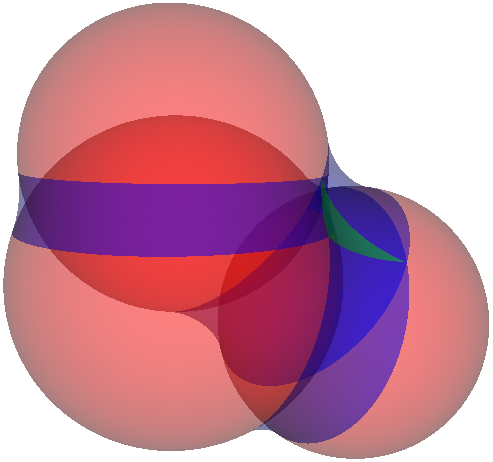
\includegraphics[width=1.5in]{image/cb-krone.png}
   % \caption{The original method \cite{krone2011parallel} rendered with transparency.}
	%	\label{fig:cb-krone}
  \end{subfigure}%
  ~
  \begin{subfigure}[t]{0.48\columnwidth}
    \centering
    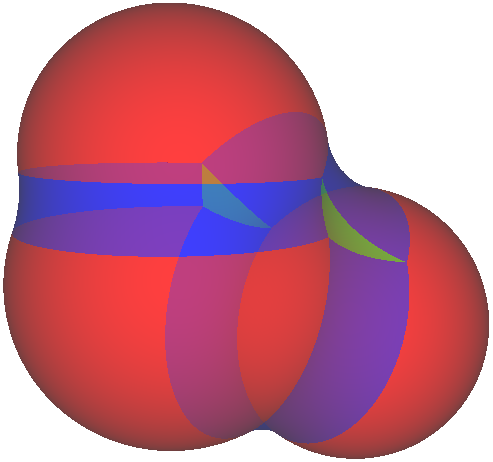
\includegraphics[width=1.5in]{image/cb-oit.png}
		%\label{fig:cb-oit}
  \end{subfigure}
	
\caption{Comparison between the original method~\cite{krone2011parallel} rendered with transparency (left) and our extended method (right).
%The transparent SES of three atoms produced by the original parallel CB algorithm (a), and our extended algorithm (b). 
The original method renders parts of spheres (red) and tori (blue) that lie below the surface.
Our method produces only patches that are part of the surface.
%More, our algorithm is also able to handle patches on a sphere that form different surfaces, i.e., the outer and one or more inner.
}
\label{fig:cb-oit}
\end{figure}

In comparison with the previous solution our main contribution here lies in the computation of toroidal and spherical patches.
Using them we avoid the situation when the previous algorithm renders the parts of tori and spheres which do not form the final surface (Fig.~\ref{fig:cb-oit}).


%Regarding tori, Kauker et al.~\cite{kauker2013rendering} proposed to ray-cast a toroidal patch using a torus and two clipping planes defined by its delimiting triangles.

%\begin{figure}[htp]
%  \centering
%  \begin{subfigure}[t]{0.55\columnwidth}
%    \centering
%    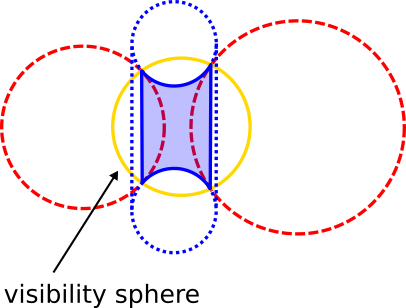
\includegraphics[width=1.7in]{image/torus-vs.png}
%    \caption{Clipping by \textit{visibility sphere}.}
%		\label{fig:torus-vs}
%  \end{subfigure}%
%  \quad
%  \begin{subfigure}[t]{0.4\columnwidth}
%    \centering
%    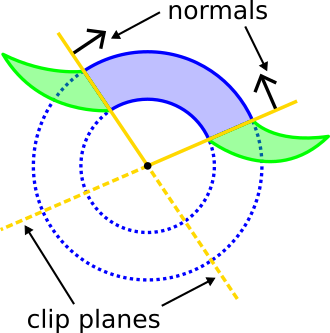
\includegraphics[width=1.3in]{image/torus-planes.png}
%    \caption{Clipping by planes defined by spherical triangles.}
%  \end{subfigure}
%\caption{Ray-tracing of a toroidal patch. The saddle part of the torus (a) is cut by so called \textit{visibility sphere}.
%A patch (b) is cut from the whole toroidal ring by clipping planes.}
%\end{figure}

%We employ his approach and modify the data structure that is used in the original algorithm to store spherical triangles in such a way that we are able to obtain all triangles incident to a torus.
%In this way, we ray-cast toroidal patches directly instead of tori.
%In order to get all neighboring triangles for a torus, we hash the triangles by three keys -- one for each torus which is connected to a triangle.
%For this, we implemented a simple hash table (see Figure~\ref{fig:hashing}) which is based on linear addressing scheme \cite{alcantara2011efficient}.

%\begin{figure}[htb]
%  \centering
%  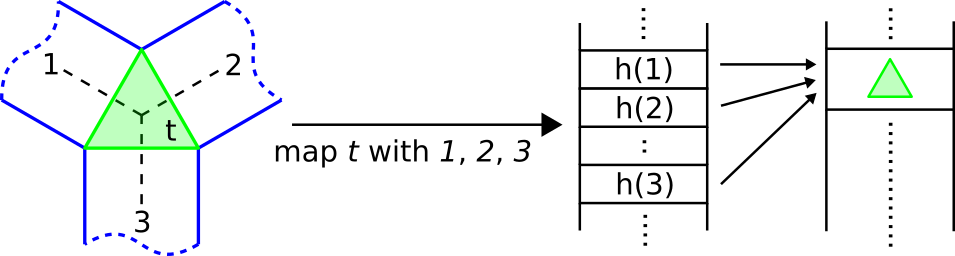
\includegraphics[width=3.3in]{image/hashing.png}
%  \caption{Our novel data structure for storing spherical triangles. Triangles $t_1$ and $t_2$ are stored linearly in an array and their incident torus $\tau$ is connected to them using a hash table.}
%	\label{fig:hashing}
%\end{figure}

To be able to compute the toroidal patches, we employ a hash data structure that enables us to store and retrieve all spherical triangles incident to a torus (Fig.~\ref{fig:hashing41}). 
%In order to get all neighboring triangles for a torus, 
We hash the triangles by three keys; i.e., one for each torus which is connected to a triangle.
For this purpose, we implemented a simple hash table, which is based on linear addressing scheme~\cite{alcantara2011efficient}.
We compute toroidal patches on a torus by retrieving all its neighboring triangles and sorting them relatively by their angular position around the torus axis.
\textcolor{green}{
Since the number of neighboring triangles of a torus is low -- for the molecule with {\tweakedsim}10000 atoms we had maximum of 8, we employ the bubble sort algorithm for this sorting.
}
When sorted, the pairs of neighboring triangles define the toroidal patches and corresponding edges.
Additionally, we check whether the first two triangles form a visible patch.
If not, then the first triangle forms a visible patch with the last one and we rotate the sorted list of triangles by one item.

\begin{figure}[htb]
  \centering
  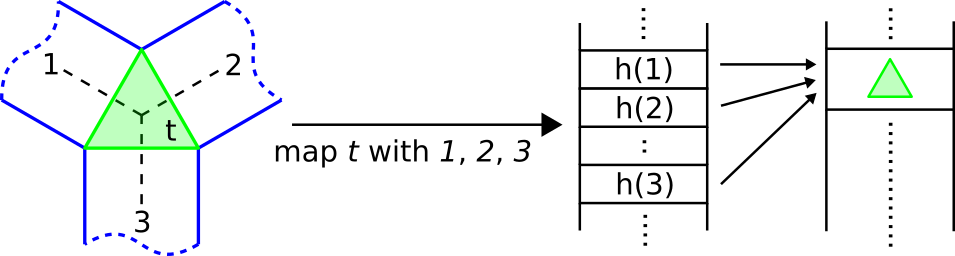
\includegraphics[width=3.3in]{image/hashing.png}
  \caption{Illustration of the data structure for storing spherical triangles. Triangles $t_1$ and $t_2$ are stored linearly in an array and their incident torus $\tau$ is connected to them using a hash table.}
	\label{fig:hashing41}
\end{figure}

This allows us to ray-cast the toroidal patches separately instead as the whole tori.

As described, a spherical patch is bounded by toroidal patches (Fig~\ref{fig:graph}). 
We extend the surface computation algorithm by adding three new GPU kernels that compute the sets of toroidal patches forming the spherical patches (see Section~\ref{sec:graph}).
When rendering the surface, each such a set is used to ray-cast a spherical patch (see Section~\ref{sec:spherical-patches}).

%\begin{figure}[htb]
%  \centering
%  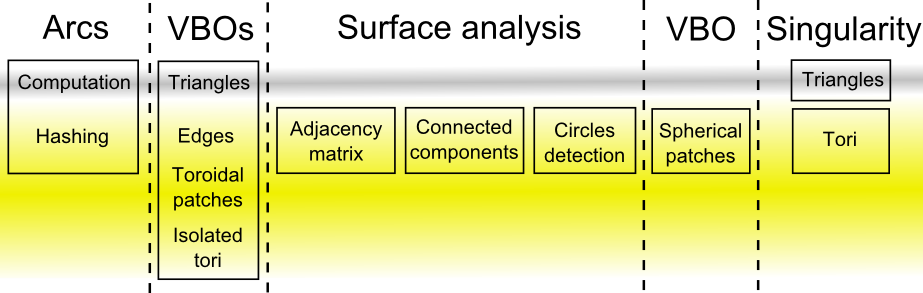
\includegraphics[width=3.3in]{image/kernels.png}
%  \caption{Overview of our extended algorithm.
%	The algorithm steps are ordered from the left to the right.
%	GPU kernels are marked with squares containing both original (grey) and our novel parts (yellow).}
%	\label{fig:kernels}
%\end{figure}

%Surface graph
\subsection{Cavity computation}
\label{sec:graph}
   
%\begin{itemize}
%  \item Idea: computed surfaces are continuous (closed) and graphs of their primitives form isolated components in the whole graph of all surface primitives
%  \item Modification of parallel CB of Krone et. al --- aaaa
%  \item Extension of parallel CB of Krone et. al --- 3 new kernels:
%	\begin{enumerate}
%	  \item Adjacency matrix is built (only 3 edges at each vertex)
%    \item Labeling of connected components (parallel BFS --- suboptimal)
%    \item Circles of edges for each spherical patch are computed
%  \end{enumerate}
%  \item Assign spheres with edges
%  \item Detect circles in edges --- bubble sort $O(n^2)$
%  \item Step 3 --- one sphere can form two or more surfaces
%  \item Rendering of spherical patches --- spherical polygons
%  \item Odd-even rule + point outside polygon
%  \item Special case: isolated tori
%\end{itemize}

The computed surface contains patches of both the outer molecular surface and the surfaces of inner cavities.
%\footnote{\textcolor{red}{JP: This should be written in more friendly fashion and with clear defined terms. Terms to be explained: surface is continuitous (geometrical?, since $C^1$ continuous it is not), graphs (2D/3D, does it contain loops?), primitive, component}}
Kauker et al. \cite{kauker2013rendering} aimed at visualizing the outer surface solely.
%\footnote{\textcolor{red}{AJ: Maybe, this could be part of related work}}
Therefore, they call the inner parts of the surface as inner remains as they represent the source of occlusion.
However, in our case we focus on the visualization of inner cavities.
%because of their significant role in the reactivity of the molecule.
%We think that for SES, the user might want to visualize cavities within the molecule and hence it is useful to let him decide on what to visualize.
Additionally, it is advantageous for the user to have the option to visualize both molecular surface and inner cavities and interactively alter between both of them; i.e., the cavities can be shown or hidden on demand.
%Contrary, for SAS, the cavities are visualized much smaller than in the case of SES and therefore visualizing them does not help assessing their shape or volume.
%The difference \textcolor{red}{stems from} the definitions of the surfaces.
%In the case of SAS, we therefore propose to clip the inner surfaces to enhance the visualization.

%The user might also want to hide cavities inside a SES to lower possible occlusion of other structures such as tunnels or cartoons.

\begin{figure}[htb]
  \centering
  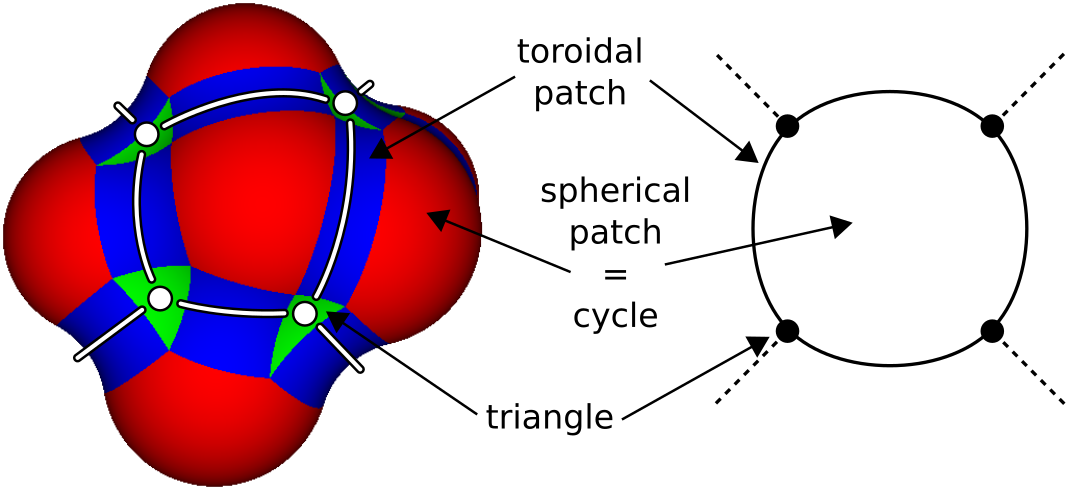
\includegraphics[width=3.3in]{image/graph.png}
  \caption{The surface graph.
	Triangles form vertices and toroidal patches form edges between them.
	Spherical patches are represented as cycles in the graph.}
	\label{fig:graph}
\end{figure}

Hiding the cavities is straightforward, since their surface is completely separated from the molecular surface.
%\textcolor{red}{\cite{borland2011ambient}}.
%\footnote{\textcolor{red}{JP: Too many ideas in one sentence. Split into two or more.}}
More specifically, one component represents the outer molecular surface and each single cavity corresponds to another component.
%For the contour representation of the surface, 
Such independent components can be easily detected by applying connected component (CC) analysis to a structure which we call the \textit{surface graph}.
%\footnote{\textcolor{red}{JP: Introduce here "terminus techniques"; i.e., SES is composed of three types of patches etc.}}
We define the surface graph using the triangles representing vertices and toroidal patches representing edges 
%since each toroidal patch is delimited by two triangles\
(Fig.~\ref{fig:graph}).
\textcolor{green}{
Then, all the vertices in the graph are of degree three.
In fact, the surface graph is an analogy to the graph of contours that define the patches.
}
%\footnote{\textcolor{red}{I don't understand the following sentence. What is former graph representation? The whole sentence should be rewritten.}}
%Moreover, using the former graph representation makes also the implementation of used graph algorithms and graph data structures on the GPU easier.

Finally, the surface contains also tori that are not delimited by any triangles.
We call these tori \textit{isolated} since they do not have any neighboring triangles (Fig.~\ref{fig:isolated-hole}).
The isolated tori are excluded from the surface graph and are handled later in the computation (see Sec.~\ref{sec:isolated}).

%\subsubsection{Extraction of surfaces}

%To extract the surfaces, i.e., the outer surface and the surfaces of the cavities, we build a \textit{surface graph} from the computed surface and apply the CC analysis to it.
The whole computation is done on the GPU in order to avoid additional data transfers between the main memory and the graphics card.
%\footnote{\textcolor{red}{Input, output}}
We split the analysis of the surface into three steps:

\begin{enumerate}
  \item Building the adjacency list of surface graph $G = (E, V)$.
	\item Finding all connected components of $G$.
	\item Finding cycles in $G$ that represent patches on spheres.
\end{enumerate}

For each step, we introduce a GPU kernel implemented as a GLSL compute shader.
%In details, our algorithm works as follows.
%First, we modified the output of the original GPU parallel CB to obtain the input which is needed for the analysis and rendering of transparent toroidal patches.

First, we build the adjacency list of $G$ from the set of edges $E$.
\textcolor{green}{We store the adjacency list of $G$ as a $|V| \times 3$ matrix since each vertex has three neighbors.}
%To build $G$, we utilize the hash table of triangles.
In fact, $E$ is prepared earlier in the surface computation phase, when we compute toroidal patches for ray-casting.
To compute these patches, we determine their delimiting triangles, thus knowing incident vertices of edges of $G$.
%\textcolor{red}{In the hash table, each triangle is hashed using all three pairs of spheres -- $(i, j)$, $(i, k)$ and $(j, k)$ that produced it.
%To retrieve a triangle for a torus, we query the hash table with a pair of its neighboring spheres as a key.}
%and therefore we also write edges for these patches into $E$.
For each non-isolated toroidal patch an edge $e$ is added to $E$ by writing its incident vertices into a buffer of edges.
%Here, we find the incident vertices of $e$ by querying the hash table of triangles.
%In the original algorithm \cite{krone2011parallel}, an arc intersection was stored only for atoms whose indices fulfilled $i < j < k$.
%This is insufficient for rendering the toroidal patches transparent as they can't be rendered as a one whole patch because the parts that would be hidden by the opaque surface would be visible.
%Instead, we split each torus into its visible patches based on their neighboring triangles that delimit them.
%Since each torus is defined by a small circle between atoms $i$ and $j$, we are interested in all triangles that were produced by atoms $i$, $j$ and some other atom $k$.
%\textcolor{red}{For this purpose, we store the computed arc intersections in a linear buffer (employing atomics) and together produce a hash structure which enables us to find the triangles by their two of the three atom indices.
%Consequently, we save GPU memory because the original arcs structure was sparse (see Appendix ?).
%Now, we store n arcs together with $3 n$ keys in a hash table which data/free ratio is 2. \textcolor{red}{TODO: More precision.}}
The first kernel then transforms the buffer of edges $E$ into a matrix representing the adjacency list of $G$.
\textcolor{green}{The matrix uses one row for each vertex $v \in V$ to store its neighbors as indices into the buffer of vertices $V$.}
%The matrix contains one row for each vertex, i.e., triangle, and three columns for its three neighbors, i.e., toroidal patches.%, because each triangle has exactly (at most?) three neighboring toroidal patches in the surface.

In the second step, all connected components of $G$ are found and labeled using the breadth-first search (BFS) algorithm.
%Our implementation of the BFS algorithm is suboptimal, because its time complexity is $O(d \cdot n)$ where d is the length of the longest shortest path among all vertices in a component.
%In the worst case, d can be n.
We opt for a simple, quadratic-work implementation~\cite{merrill2012scalable}, because of the ability to have the BFS implemented in a single kernel.
Our decision is supported by the performance measurements (see Sec.~\ref{sec:performance}) where the computation of surface components takes {\tweakedsim}5 ms for a molecule with {\tweakedsim}10.000 atoms while the computation of SES and its ray-casting together takes {\tweakedsim}41 ms.

In the last step, the cycles representing the spherical patches are extracted.
To do this, we assign the edges in $E$ by their neighboring spheres into buckets.
We then order the edges in buckets by their adjacency, so that they represent one or more cycles in $G$.
A spherical patch is labeled by the label of any of its delimiting edges.

\subsubsection{Special case -- Isolated torus}
\label{sec:isolated}

We handle the isolated tori in two steps.
First, a label for a torus is retrieved. 
Note that an isolated torus is not part of the surface graph.
Second, for each isolated torus, we clip fragments in its neighboring spherical patches that are overlaid by the torus. 
Otherwise, these fragments would create a false surface layer between a torus and a spherical patch (Fig.~\ref{fig:isolated-hole}).

\begin{figure}[htp]
  \centering
  \begin{subfigure}[t]{0.55\columnwidth}
    \centering
    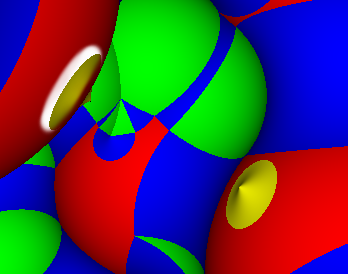
\includegraphics[height=1.4in]{image/isolated-cutaway2.png}
    %\caption{An \textit{isolated} torus.}
		%\label{fig:isolated-cutaway}
  \end{subfigure}%
  \quad
  \begin{subfigure}[t]{0.4\columnwidth}
    \centering
    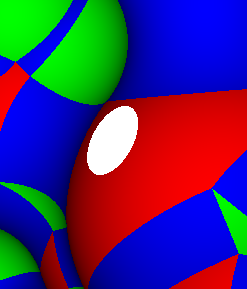
\includegraphics[height=1.4in]{image/isolated-hole.png}
    %\caption{A hole in a spherical patch.}
  \end{subfigure}
\caption{Example of an isolated torus between two spheres.
	Left: Isolated tori (yellow) do not have neighboring triangles, therefore the surface component to which they belong cannot be determined directly from the surface graph. Right: An isolated torus cuts circular holes into its neighboring spherical patches.}
\label{fig:isolated-hole}
\end{figure}

An isolated torus can be encountered while writing the toroidal patches for ray-casting.
We add this torus into the buffer for ray-casting and we also mark it for later processing.
Later on, when the detection of surface components is done, we run another kernel which assigns the isolated tori to their surface labels.
The assignment is done by inspecting the neighboring spheres of the tori.
There can be two cases:
\begin{enumerate}
  \item One of the spheres forms only one patch. Then the torus lies in the same surface component as this patch.
	\item Both spheres form two or more patches. We find a neighboring patch of the torus by employing the point in a spherical patch test (see Section~\ref{sec:spherical-patches}). Then the torus lies in the same surface component as its neighboring patch.
\end{enumerate}

The clipping of fragments in the affected spherical patches can be done using a clipping plane or \textit{visibility sphere} (\textcolor{green}{introduced in~\cite{krone2009interactive}}) of a torus.
We use the latter approach, since the visibility spheres for tori were already computed in a previous phase of our technique.
Here, our kernel writes a texture, similarly to Krone et al.~\cite{krone2011parallel}, which stores all visibility spheres that intersect the sphere.
When ray-casting spherical patches, we use this texture to discard all fragments that are inside of the intersecting visibility sphere.


\section{Visualization}
\label{sec:vis}

To enable our focus and context transparent visual, we require an ordered list of fragments for each screen pixel. This list of fragments is also commonly referred as an A-buffer. We implemented the A-buffer using per-pixel linked lists~\cite{yang2010real}. In our case, the A-buffer fragments represent three types of surface patches analytically computed for a given ray.

\subsection{Ray-casting}
\label{sec:spherical-patches}
To form fragments of each surface patch we employ a ray-casting technique. To provide a high performance, the ray-patch intersection is computed analytically.
In 2013, Kauker et al.~\cite{kauker2013rendering} proposed to ray-cast a toroidal patch using a torus and two clipping planes defined by its delimiting triangles (Fig.~\ref{fig:torus-vs}).
\begin{figure}[htp]
  \centering
  \begin{subfigure}[t]{0.55\columnwidth}
    \centering
    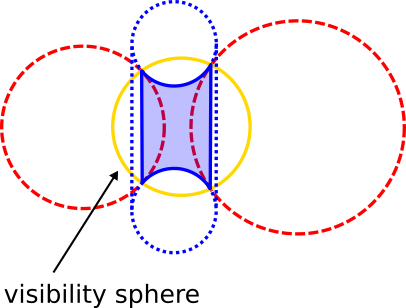
\includegraphics[width=1.7in]{image/torus-vs.png}
    \caption{Clipping by \textit{visibility sphere}.}
		\label{fig:torus-vs}
  \end{subfigure}%
  \quad
  \begin{subfigure}[t]{0.4\columnwidth}
    \centering
    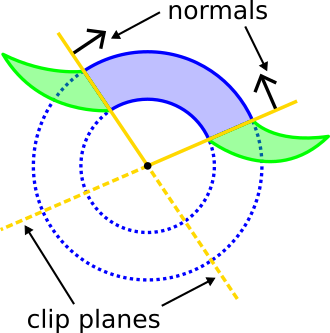
\includegraphics[width=1.3in]{image/torus-planes.png}
    \caption{Clipping by planes defined by spherical triangles.}
  \end{subfigure}
\caption{Ray-tracing of a toroidal patch. The saddle part of the torus (a) is cut by so called \textit{visibility sphere}.
A patch (b) is cut from the whole toroidal ring by clipping planes.}
\end{figure}

We employ this approach and, moreover, we modify the data structure being used in the original algorithm to store and retrieve all spherical triangles incident to a torus (Fig.~\ref{fig:hashing}). In order to get all neighboring triangles for a torus, we hash the triangles by three keys; i.e., one for each torus which is connected to a triangle.
For this purpose, we implemented a simple hash table, which is based on linear addressing scheme \cite{alcantara2011efficient}.
\begin{figure}[htb]
  \centering
  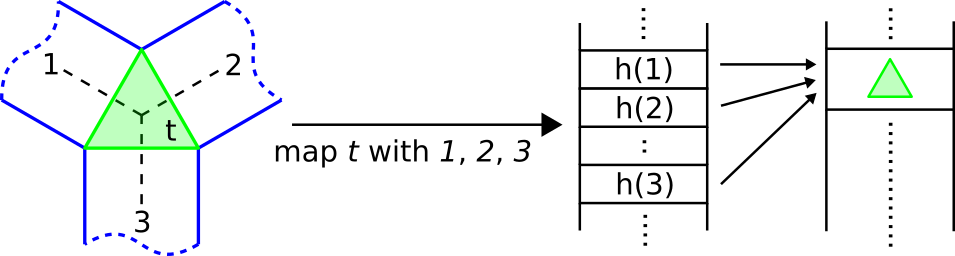
\includegraphics[width=3.3in]{image/hashing.png}
  \caption{An illustration of the data structure for storing spherical triangles. Triangles $t_1$ and $t_2$ are stored linearly in an array and their incident torus $\tau$ is connected to them using a hash table.}
	\label{fig:hashing}
\end{figure}
This allows us, to ray-cast toroidal patches directly instead of tori.


Ray-casting the sphere is a trivial task; nevertheless, in our case the surface sphere of molecules might be formed by an arbitrary number of spherical patches lying in different surface components. To avoid obvious rendering issues, i.e., distinct coloring, transparency or visibility, we perform ray-casting of each spherical patch separately.
This allows us to visually distinguish between different surface components.

Since the boundaries of a spherical patch are formed by small circle arcs, we apply an odd-even rule for polygons~\cite{shimrat1962algorithm} to test whether a point lies inside the patch. Firstly, we compute intersection points, $P_{front}$ and $P_{back}$, of a given ray with the patch sphere.
Here, we describe the point-patch test for point $P_{front}=P$ only, since the same test is applied to $P_{back}$.
Before we apply the odd-even rule, we choose a point $O$ lying outside the patch.
Then, we test line $OP$, the shortest path on a sphere, for an intersection with each of the arcs delimiting the patch.
The intersection of a line $OP$ with the small circle arc, given by points $AB$, is computed in two steps (Fig.~\ref{fig:outer-point}a):
\begin{enumerate}
  \item Intersections of the circles containing the line and the arc, which can intersect in up to $2$ points.
  \item Intersection points are tested whether they belong to both the segment $OP$ and the arc $AB$.
\end{enumerate}
Finally, if the sum of all intersections, i.e., for all the sides, is even then the point lies inside the patch.

\begin{figure}[htp]
  \centering
  \begin{subfigure}[c]{0.52\columnwidth}
    \centering
    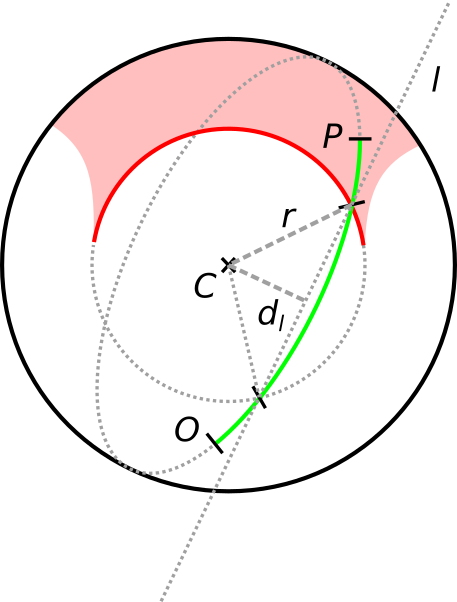
\includegraphics[height=1.9in]{image/patch.png}
    \caption{%Point in spherical patch test.
		The intersection $I_1$ lies on an intersection line between two planes containing arcs $OP$ and $AB$.}
		\label{fig:spherical-patch}
  \end{subfigure}%
  \quad
  \begin{subfigure}[c]{0.44\columnwidth}
    \centering
    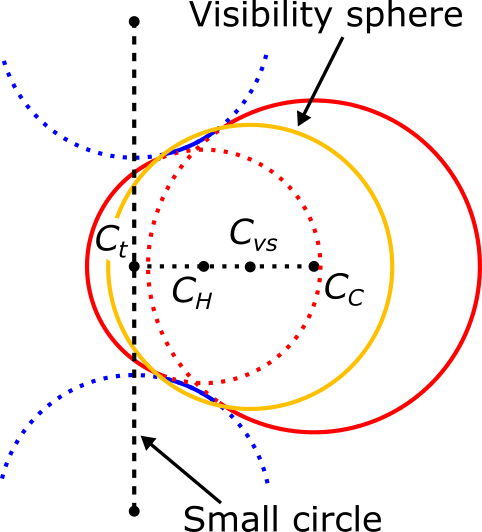
\includegraphics[height=1.6in]{image/outer.png}
    \caption{%A torus formed by carbon ($C_C$) and hydrogen ($C_H$) atoms.
		The center of the torus ($C_{t}$) lies outside the atom centers, while the center of its visibility sphere $C_{vs}$ lies between $C_C$ and $C_H$.}
		\label{fig:outer-point}
  \end{subfigure}
\caption{Point in spherical patch test (a). A torus formed by carbon ($C_C$) and hydrogen ($C_H$) atoms (b).}
\end{figure}

Since we deal with spherical patches and not the planar ones, the situation is bit more complex and we cannot choose point $O$ arbitrarily. 
%Otherwise, we would count intersections of patch's sides with a great circle containing $P$.
%Then, the intersection count would be the same regardless of $P$ being inside or outside the patch, making the rule inapplicable.
Instead, we compute $O$ by intersecting a patch sphere by an axis of one of its delimiting tori.
In this way, we get two intersection points from which we choose the one that lies in the direction of the torus visibility sphere (Fig.~\ref{fig:outer-point}).

%\subsection{Ambient Occlusion Opacity Modulation}
%Borland~\cite{borland2011ambient} proposed to utilize ambient occlusion (AO) values to alter the opacity. Motivated by his approach, we exploit the ambient occlusion values as well. Since, we would like to maintain fast rendering performance, we need to remedy the issue of having an object space technique to evaluate the AO values. In the former work of Borland, the performance was considered a less important factor, which allows him to exploit the full object space AO evaluation. Here, we opted for the most recent approach, proposed by Grottel et al.~\cite{grottel2012object}, which renders ambient occlusion values to a $3D$ grid containing an estimate of the volume area of atoms located inside a voxel. Although this approach only reflects the volume of atoms and not the volume area of the molecular surface, we find it as a good trade off between the visual precision and the performance measure. Note, in addition, these values are not employed directly, but rather as opacity modulators instead, which defines the opacity as follows:
%\begin{equation}
  %\alpha = \left( \frac{O}{\tau}\right)^\rho,
	%\label{eq:alpha}
%\end{equation}
%where $\tau$ represents a threshold such that $alpha=1$ if $O\geq\tau$. Moreover, the resulting $\alpha$ values are clampled to interval $[0,1]$. An example of comparison between different $\tau$ values is depicted in Figure~\ref{fig:TODO}.
%
%Another property we propose to use as the opacity modulator is the surface area of the cavity (TODO do we use this as well, or just using colors?).
%\begin{figure}[htb]
%\centering
  %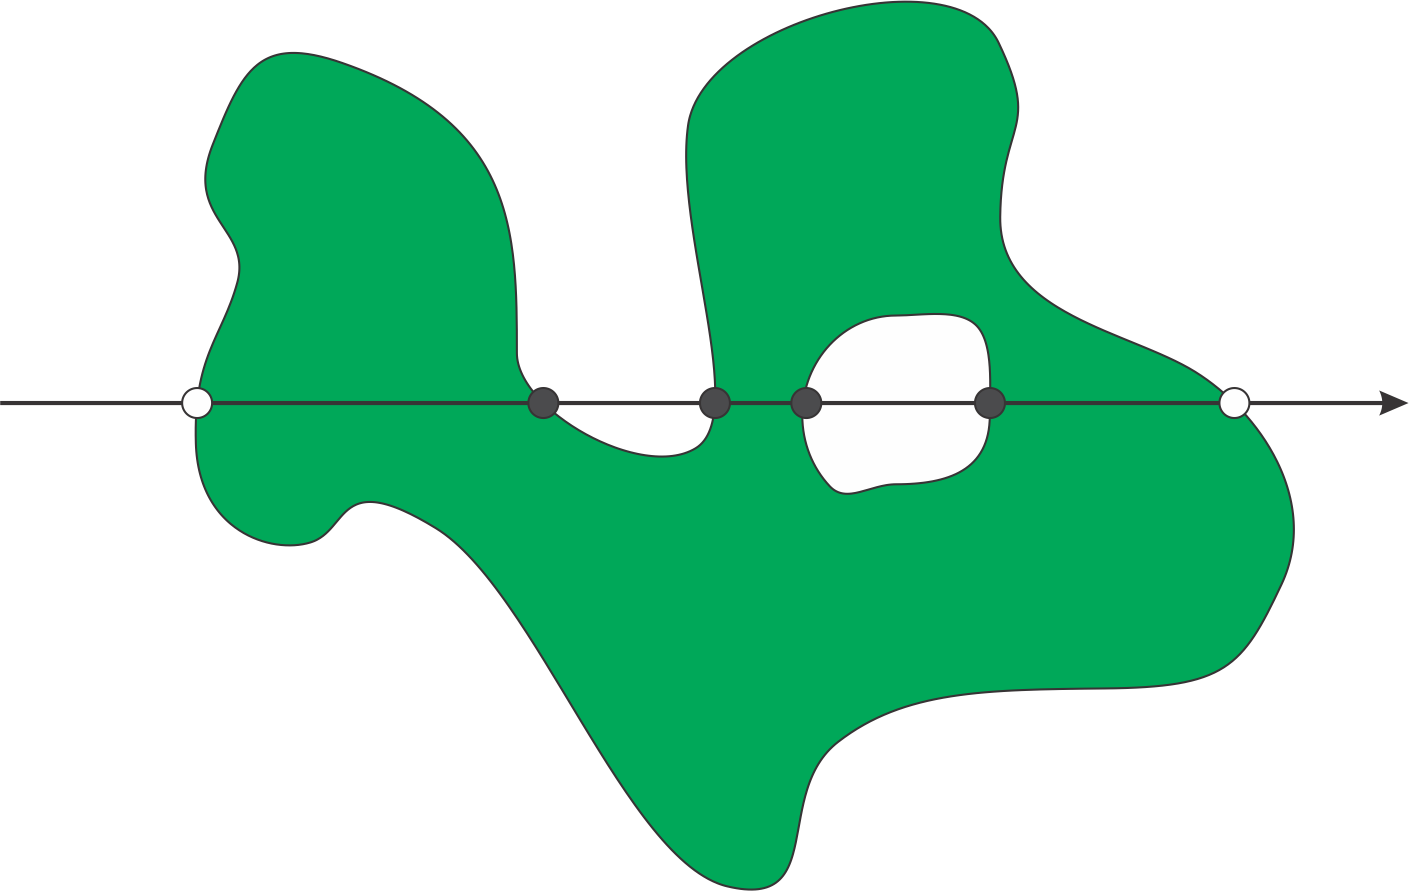
\includegraphics[width=0.8\columnwidth]{image/ray_fragments.png}
  %\caption{(TODO make more nice with overlay AO grid). An example of the list of fragments per a given ray. The color of the circles represent the obtain ambient occlusion value.}
	%\label{fig:ray_fragments}
%\end{figure}

\subsection{Opacity modulation}
After the intersection points were computed, we sort, in front-to-back manner, and store them in the linked list. Thus, for a given ray, we acquire a list of fragments $\{f_1,\ldots,f_n \}$, where each pair represents an entry and an exit point for the molecular surface. For simplicity, the values of $f$ represent depths of fragments. We denote the entire distance the ray passes through the molecule as $l=|f_1-f_n|$. 
As we step along each fragment $f_i$, we define the opacity $\alpha_i$ of even fragments, i.e., those representing the entry surface points, as follows:
\begin{equation}
  \alpha_i = O^{\phi(x)},
	\label{eq:alphaDistEven}
\end{equation}	
where $O$ represents a user defined parameter affecting the overall opacity and $\phi(x)$ suppress or amplifies the opacity and is defined as
\begin{equation}
  \phi(x) = K-(K-1)x,
	\label{eq:exponent}
\end{equation}	
where $K$ is the maximum value of the exponent and $x=|f_{i+1}-f_i|/l$ represents the ratio of the fragment interval to the entire length $l$. Note that if $x=1$, i.e., having just two fragments on the ray, then $\phi(x)=1$ determining the $\alpha_i=O$. The opacity of odd fragments, i.e., representing the exist surface points, is defined as $\alpha_i = O$, thus keeping them unmodulated since they are less prominent in the final image.
Figure~\ref{fig:Oparam} showcases $4$ different combinations of parameters $K$ and $O$.
\begin{figure*}[htb]
  \centering
  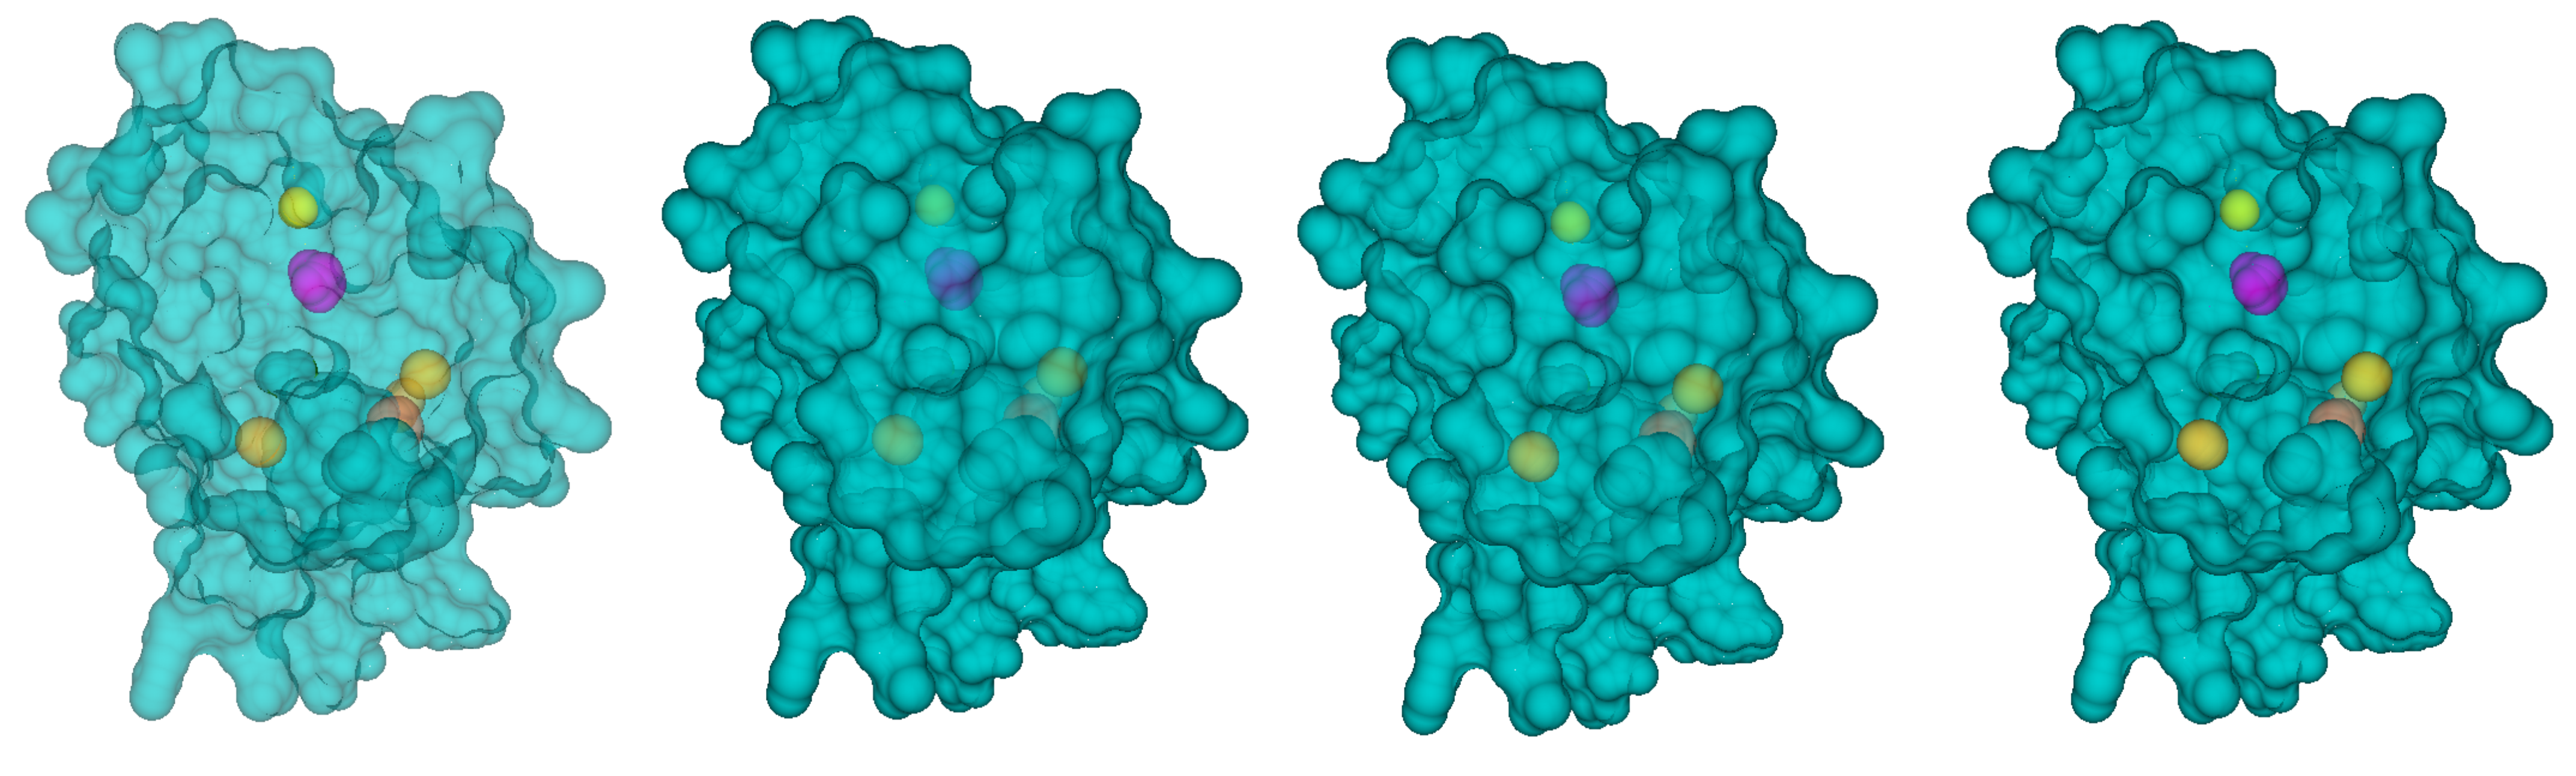
\includegraphics[width=\textwidth]{image/Oparam.png}
  \caption{An example of application of parameters $K$ and $O$ on protein $1cqw$. Note that higher values of the overall opacity $O$ emphasize the front molecular surface, while higher values of maximum exponent $K$ give more prominence to the internal surfaces and cavities.}
	\label{fig:Oparam}
\end{figure*}
\subsection{Cavity area estimation}
We enhance the visualization of cavities by coloring their surface by their approximate areas.
To estimate the area, we sum areas of all triangles that form the cavity surface.
The area of a spherical triangle is calculated as follows:

\begin{equation}
  S = r_{probe}^2 \left[ \left( A + B + C \right) - \pi \right],
\end{equation}

where $A$, $B$ and $C$ are angles of the triangle. 
%We do the area computation in a GLSL compute shader which computes areas of individual triangles and sums them using atomics.
Additionally, we neglect areas of spherical and toroidal patches since their influence on the exact cavity area is much smaller compared to triangles.
%Therefore, the cavity area we compute is \textcolor{red}{underestimated -- maybe an equation?}.
Naturally, this observation does not hold for the molecular surface.
%\textcolor{red}{What about coloring?}


\section{Discussion}
The contribution of our proposed system will be demonstrated on a case study which corresponds to real problems the biochemists are currently facing. 
Later, we present the detailed performance analysis.

\subsection{Case Study~--~Real-time visual exploration of MD simulation}
The case study deals with the situation when the biochemists want to visually explore the inner processes occurring inside the molecule. 
An example of such a process can be the penetration of a small molecule (ligand) into the active site of the protein where the ligand reacts with the protein and the product of such reaction can form the basis of new chemical matters, e.g., new drugs. 
The current workflow generating the desired visual appearance of the animation showing such processes consists of many trial and error attempts, which makes the whole workflow very lengthy. 
To describe this process in more detail, the biochemists start in the first time step of the whole simulation and try to manually determine the best viewpoint.
As the view inside the molecule, where the processes usually occur, is crucial, they utilize clip planes to achieve this.
The manual setting of the clip planes introduces other possible error to the final animation.
The dynamic movements of the molecule can cause its rotation and the clip plane settings in the first time step might have completely wrong positions in the following steps .
When all the visual parameters are set in the first frame (Fig.~\ref{fig:animation}), the biochemists use an offline rendering tool for generating the whole animation.
In this phase they do not posses any control of this process so it is impossible to detect an error inside the animation and stop the generation.
These errors, such as occlusions or wrong clip plane positions, are detected when playing the final animation.
The only solution is to adjust the input settings and launch the whole process once again.
For better illustration, in case of the example video (from which Figure~\ref{fig:animation} (top) is captured), it took two days to produce the solution which comprehensibly shows the whole process of ligand penetration to the protein active site.

Our new system is able to overcome the following limitations of the above-described workflow:
\begin{itemize} 
\item The MD simulation can be observed in real time which enables the user to interactively adjust the appearance and viewpoint.
\item The highly transparent molecular surface removes the necessity of using clip planes.
\item The user has the full control of the animation process so we completely remove the trial and error phase of the workflow. 
\end{itemize}

In consequence, our system enables to reach similar results in real-time. 
In one aspect it even overcomes the existing solution as the users can interactively manipulate with the scene on the fly~--~perform scene transformations, change the appearance of the protein and ligand, or change the probe size used for the generation of protein surface.

Figure \ref{fig:animation} (bottom) shows one time step of the animation generated using the same dataset as for the top part of this Figure.

\begin{figure}[htb]
  \centering
  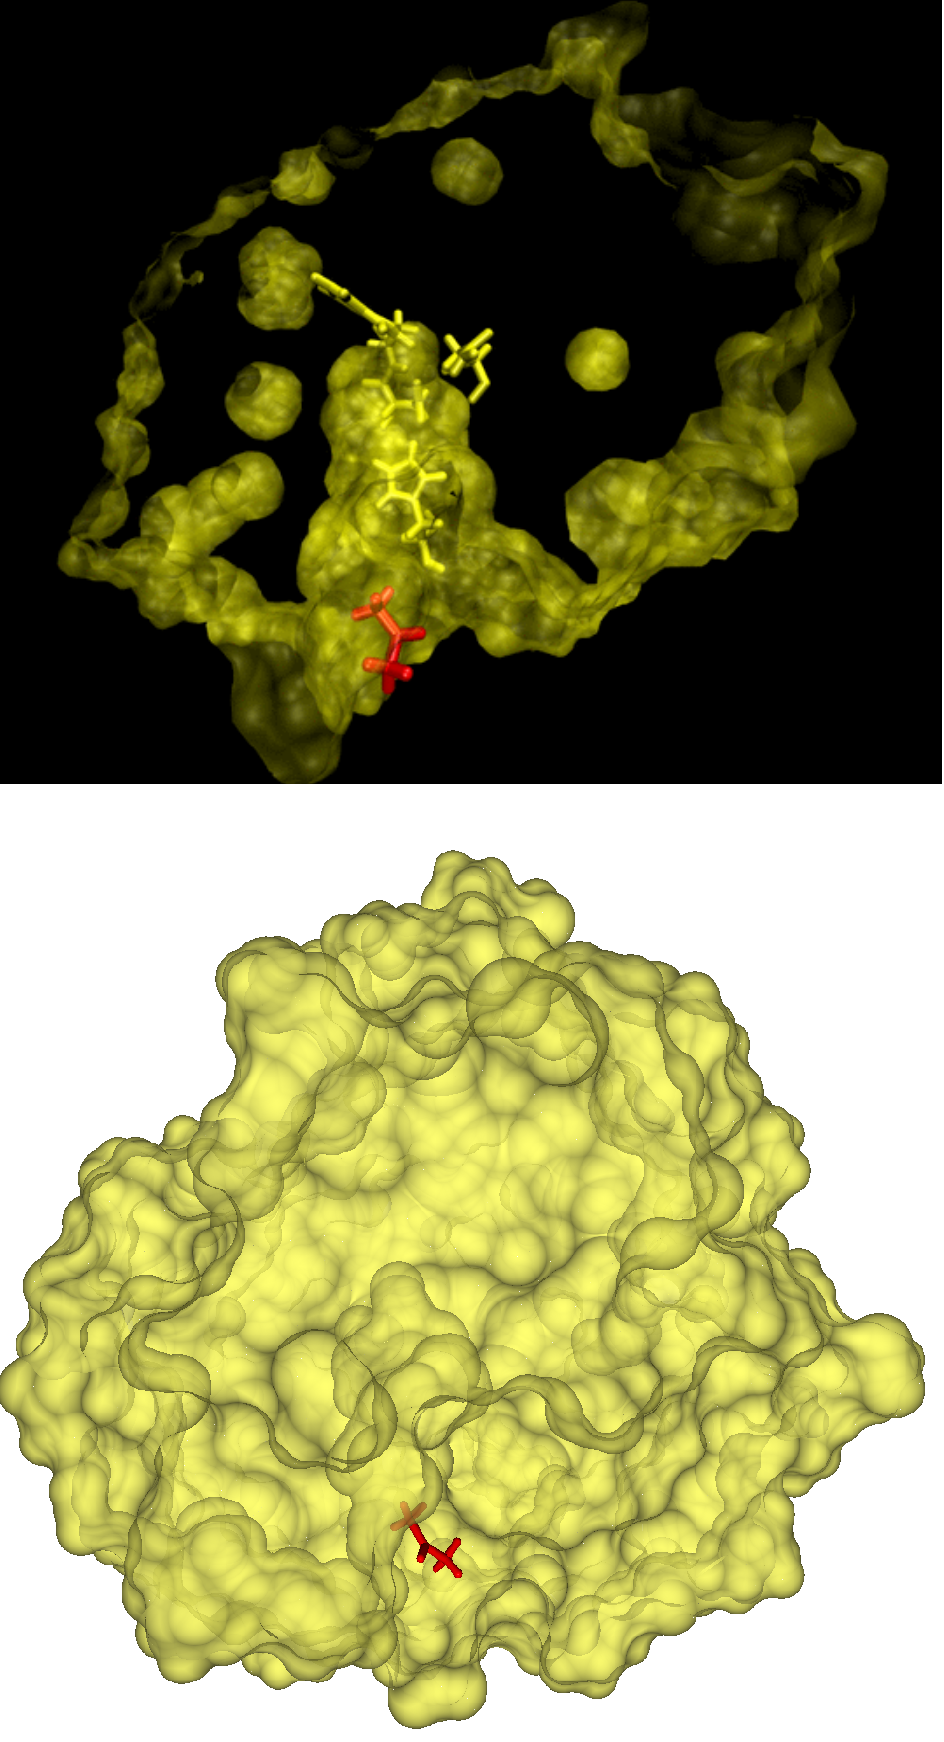
\includegraphics[width=2.5in]{image/animation.png}
  \caption{Top: One time step from the animation aiming to show the penetration of the ligand to the protein active site. For better insight, different representations of the molecule and the ligand, surface transparency, clip plane, and different coloring was used. Bottom: One time step of the animation generated using our algorithm. It shows the same molecule and its dynamics. By enabling the interactive manipulation with the scene within the animation, the user can clearly see the transportation route without the necessity to use any clip plane.}
	\label{fig:animation}
\end{figure}

When the results of the algorithm were evaluated by the domain experts, they confirmed that our solution is highly practical with respect to the described task because the time to complete this task is reduced dramatically.
Moreover, they also appreciated the visual appearance which they considered to be more appealing than the previous solutions.
They confirmed that our approach can be directly used for creating presentation materials, such as images to publications or animations for presentations.

The domain experts were also asked to identify the weak points of our current solution.
They agreed that when using a highly transparent molecular surface, the position of a ligand can be hard to assess when using only one viewpoint.
In other words, the user has to manipulate with the structure in order to decide if the ligand is still located in the outer solvent or if it already penetrated to the inner part of the protein.
However, this situation is caused due to the transparency itself and a solution has to be based on a combination with other methods.
This opens one of the possible directions for the future extension.

\subsection{Performance Analysis}
\label{sec:performance}

We tested our technique on commodity hardware to show that it enables the users to solve their tasks in real-time without high hardware requirements.
%\textcolor{red}{Test also on high-end hardware --- GTX 980?}
The tests were performed using Intel Core i5 760 (2.80 GHz) with 4 GB of RAM and NVIDIA GeForce 680 GTX with 4 GB of VRAM as a graphics card.
For rendering, we used resolution of 1024 $\times$ 768 and we tried to fit the molecule such that it covered most of the image.
Regarding transparency, we limited the maximum depth complexity to 24 fragments per pixel.
The results of our measurements for both static and dynamics molecules are presented in Table~\ref{tab:static}.
We choose the static structures from Protein Data Bank (PDB)~\cite{sussman1998protein} such that the performance of our technique could be easily compared with other existing or new approaches.

\setlength{\tabcolsep}{4.5pt}

\begin{table}[htb]
  \caption{Performance of our technique for static and dynamic (*) structures.
	The table shows timings of key phases of our method: surface computation (CB), cavity computation (SG), area estimation and ray-casting (RC).
	For ray-casting, we also include fill rate (FR).
	Performance of our technique does not vary significantly for static or dynamic data as it operates on a per-frame basis.}
  \label{tab:static}
  \scriptsize
  \begin{center}
    \begin{tabular}{cccccccc}
      Molecule & \# Atoms & FR & CB & SG & Area & RC & Total \\
			%        &       & buildup  & graph   & Area & casting &       \\
							&      & (\%) & (ms)     & (ms)    & (ms) & (ms) & (FPS) \\
    \hline
      1OGZ &  {\tweakedsim}1000 & 36.7 &  4.1 & 0.2 & 0.2 & 15.7 & 31.0 \\
      1VIS &  {\tweakedsim}2500 & 52.7 &  6.1 & 0.8 & 0.2 & 39.3 & 16.4 \\
			LINB-ACE* & {\tweakedsim}4500 & 55.4 & 17.4 & 0.6 & 0.2 & 47.6 & 12.3 \\
      4ADJ & {\tweakedsim}10000 & 41.5 & 21.1 & 4.3 & 0.4 & 97.7 &  6.9
    \end{tabular}
  \end{center}
\end{table}

%\begin{table}[htb]
%  \caption{Performance of our technique for a dynamic molecule.
%	The table shows timings of key phases of our method: surface computation (CB), cavity computation (SG), area estimation and ray-casting.
%	For ray-casting, we also include fill rate (FR).}
%  \label{tab:static}
%  \scriptsize
%  \begin{center}
%    \begin{tabular}{cccccccc}
%      Molecule & \# Atoms & FR & CB & SG & Area & Ray-casting & Total \\
%			%        &       & buildup  & graph   & Area & casting &       \\
%							&      & (\%) & (ms)     & (ms)    & (ms) & (ms) & (FPS) \\
%    \hline
%      LINB-ACE & {\tweakedsim}4500 & 55.4 & 17.4 & 0.6 & 0.2 & 47.6 & 12.3 \\
%    \end{tabular}
%  \end{center}
%\end{table}

Our technique was implemented mainly using OpenGL employing GLSL compute shaders as GPU kernels.
We also utilize OpenCL to accelerate a kernel which computes positions of spherical triangles in the original algorithm \cite{krone2011parallel}.
The GLSL implementation of this kernel performed for a molecule with {\tweakedsim}10000 atoms is about 5x slower than the OpenCL/CUDA one.
From the tests we did, we assume that the key of such performance loss is the extensive use of the global memory in the kernel which is handled differently in OpenGL and OpenCL/CUDA.

From the results, it can be seen that in terms of performance, the main limitation of our technique is ray-casting of the computed surface.
More specifically, the demanding parts are rendering of spherical and toroidal patches that take together 75-80\% of the whole rendering time.
We anticipate that the performance of ray-casting these patches could be improved by using tighter bounding boxes for them when splatting.
In fact, we employ bounding squares for both spheres containing spherical patches and visibility spheres containing visible parts of tori.
In this way, the computation of ray-primitive intersection is evaluated multiple times for spheres and tori that form more than one surface patch.

\subsubsection{Improved memory complexity}

As a side effect of exploiting the hash data structure (Sec.~\ref{sec:ecb}) for storing spherical triangles, our technique consumes less GPU memory than the approach we come from.
This is due to the fact that the original method uses a linear buffer to store spherical triangles.
An index into this buffer, i.e., position where a triangle is stored, is computed based on the $i$ and $j$ indices of spheres $i < j < k$ that formed the triangle.
The range of $j$ is optimized in terms of limiting a maximal number of neighbors ($maxNeighbors$) that a sphere can have, so that the range of $j$ can be remapped to $\left[0, maxNeighbors\right)$.
There is also a limit on a total number of triangles ($maxTriangles$) that can be stored for each pair of spheres.
Putting it all together, the memory complexity of the original data structure is:

\begin{equation}
|A| \cdot maxNeighbors \cdot maxTriangles,
\end{equation}

where $|A|$ is the number of atoms of the molecule and typical settings for the other two constants are $maxNeighbors = 64$, $maxTriangles = 64$.
We took this settings from the MegaMol visualization framework~\cite{grottel2015megamol}.

On the other hand, we store the computed triangles linearly in an array and for each triangle, we additionally store three hash records. The memory complexity of our hash structure is therefore:

\begin{equation}
|T| + hashFreeRatio \cdot 3 |T|,
\end{equation}

where $|T|$ is number of computed spherical triangles and the typical setting for the constant is $hashFreeRatio = 2$. 

To be able to compare the complexities of these two data structures, we estimate the ratio of number of atoms to number of triangles to be (taken from experiments):

\begin{equation}
\frac{|A|}{|T|} > \frac{1}{4}.
\end{equation}

Then, the ratio of complexities can be expressed as:

\begin{equation}
\frac{|A| \cdot maxNeighbors \cdot maxTriangles}{|T|(1 + 3 \cdot hashFreeRatio)} > \frac{64^2}{28} > 146,
\end{equation}

which yields that the original structure is more than 100 times larger for only 64 neighbors.
Actually, our maximum neighbor count is 128, to be able to compute surface of molecules that contain hydrogens, which is a typical case for data produced by molecular dynamics simulation.

\section{Conclusion}
Future work
\begin{itemize}
  \item More tight bounds for ray-casting may further improve the performance. This holds especially for tori because each torus is ray-casted xxx (about 2) times in average. (AJ)
  \item The ray-casting could be done using OpenCL which could lower bandwidth because the data common to many fragments could be fetched only once and shared using local (shared) memory. (AJ)
\end{itemize}

%% if specified like this the section will be ommitted in review mode
\acknowledgements{
The authors wish to thank A, B, C.}

\bibliographystyle{abbrv}
%%use following if all content of bibtex file should be shown
%\nocite{*}
\bibliography{pvis2016}

\appendix
\section{Original arcs structure vs. our hash structure size}
Orignal structure complexity is $|A| \cdot maxNeighbors^2$ where $maxNeighbors = 64$.

Our structure complexity is $|T| + hashFreeRatio \cdot 3 |T|$ where $hashFreeRatio = 2$.

The ratio of atoms to triangles is approximately (value from experiments) $\frac{|A|}{|T|} > \frac{1}{4}$ so that $\frac{|A| \cdot maxNeighbors^2}{|T|(1 + 3 \cdot hashFreeRatio)} > \frac{64^2}{28} > 146$ which means that the original structure is more than 100 times larger for only 64 neighbors. Actually, our maximum neighbor count is 128, to be able to compute surface of molecules that contain hydrogens.

http://idav.ucdavis.edu/\~dfalcant/downloads/dissertation.pdf

\end{document}
